\documentclass[11pt]{book}
\usepackage{longtable}
\usepackage{color}
\usepackage{tabu}
\usepackage{setspace}
\usepackage{pdflscape}
\usepackage{graphicx}
\usepackage {float}
%\usepackage{subfigure}
\usepackage{caption}
\usepackage{subcaption}
\usepackage{natbib}
\usepackage{fullpage}
\bibliographystyle{plain}
%\bibliographystyle{cbe}
\usepackage{algorithmic}
\usepackage[vlined,ruled]{algorithm2e}
\usepackage{amsmath}
\usepackage{amsfonts}
\usepackage{amssymb}
\usepackage[T1]{fontenc}
\usepackage{url}
  
\usepackage[dvipsnames]{xcolor}
\usepackage{color, soul}
\usepackage[colorlinks=true, linkcolor=blue, citecolor=DarkOrchid, urlcolor=TealBlue ]{hyperref}
%\usepackage[nottoc,numbib]{tocbibind}
\usepackage{tocloft}

\setlength\itemindent{1cm}

\newcommand{\phyg}{\texttt{PhyG} }
\newenvironment{phygdescription}{\subsubsection{Description}}{}
\newenvironment{example}{\subsubsection{Examples} \begin{itemize}}{\end{itemize}}
\newenvironment{argument}{\subsection{Arguments}\begin{itemize}}{\end{itemize}}
%\item [ ]

% We define a command environment for new command definitions, and store
% whatever command we are dealing with in the @commandname macro. Inside a
% command we can specify the defaults, the syntax, and the arguments to be used.
    \newenvironment{command}[2]{
	\def\tmpa{}
	\def\tmpb{#2}
	\def\@commandname{#1}
	\subsection{#1}\index{general}{#1}
	\ifx\tmpa\tmpb 
	\label{comm:#1} 
	\else 
	\label{comm:#2} 
	\fi}
{}

% Syntax definition. We use the name of the command as stored in @commandname
\newcommand{\syntax}{\subsubsection{Syntax} \@commandname} 
\newcommand{\atsymbol}{@}

\begin{document}
	%\firstpage{1}
	
	\title{PhylogeneticGraph\\User Manual\\Version 0.1}
	
	\maketitle
	
	\newpage

	 \begin{center}
		
\includegraphics[width=\textwidth]{AMNHLogo.jpg}
	\end{center}

	\vspace*{5.50cm}	
	\begin{flushleft}
		\textbf {Program and Documentation} \\ Ward C. Wheeler \\
		\vspace*{0.50cm}
		\textbf {Program} \\ Alex Washburn  \\
		\vspace*{0.50cm}
		\textbf{Documentation} \\ Louise M. Crowley
	\end{flushleft}
	

	\vspace*{5.50cm}
	
	\begin{flushleft}
		\small
		{\it Louise M. Crowley, Alex Washburn,  Ward C. Wheeler} \\
		
		Division of Invertebrate Zoology, American Museum of Natural History, New York, NY, U.S.A.\\
		\smallskip
		The American Museum of Natural History\\
		\copyright  2022 by The American Museum of Natural History, \\
		All rights reserved. Published 2022.
		
		%	\vspace*{0.25cm}
		%	\emph{W. C. Wheeler.} 2022. \texttt{PHYG} 1..0. New York, 
		%	American Museum of Natural History. Documentation by W.C. Wheeler and L. M. Crowley. 
		%	
		\vspace*{0.25cm}
		
		Available online at \url{https://github.com/wardwheeler/PhyGraph.git} 
		
		Comments or queries relating to the documentation should be sent to \href{mailto:wheeler@amnh.org}
		{wheeler@amnh.org} or \href{mailto:crowley@amnh.org}{crowley@amnh.org}
	\end{flushleft}
	
	\tableofcontents

\chapter{What is PhyG?}
	\section{Introduction}
	PhylogeneticGraph (\phyg) is a multi-platform program designed to produce phylogenetic 
	graphs from input data and graphs via heuristic searching of general phylogenetic graph 
	space. \texttt{PhyG} is the successor of \href{https://github.com/wardwheeler/POY5}{\textbf{POY}}
	\citep{POY2,POY3,POY4,Varonetal2010,POY5, Wheeleretal2015}, containing much of its 
	functionality including the optimization of unaligned sequences, and the ability to implement 
	search strategies such as random addition sequence, swapping, and tree fusing. As in {\textbf{POY}, 
	\phyg can generate outputs in the form of implied alignments and graphical representations of 
	cladograms and graphs. What sets \phyg apart from {\textbf{POY}, and other phylogenetic 
	analysis programs, is the extension to broader classes of input data and phylogenetic graphs. 
	The phylogenetic graph inputs and outputs of \texttt{PhyG} include trees, as well as other forms 
	including forests and both soft- and hard-wired networks.
	%\phyg generates ...
		
	This is the initial version of documentation for the program.
	
	\section{Overview of program use}
	At present, \phyg  is operated solely via command-line in a terminal window. Commands 
	are entered via a script file containing commands that specify input files, output files and 
	formats, graph type and search parameters. Running analyses using scripts allows for the 
	entire analysis to proceed from the beginning to the end with one click of a button and 
	may produce results faster as \phyg automatically optimizes the workflow of the analysis
	by taking into account the functional relationships among various tasks and efficiently 
	distributing the jobs and resources (such as memory and multiple processors). This script 
	can also include references to other script files.

%	%\begin{figure}
%	\begin{center}
%	\includegraphics[width=0.6\textwidth]{doc/Figures/First_script.jpg}
%	\end{center}
%	\caption{\phyg script}
%	%\end{figure}
	
	\begin{figure}
	\centering
	\includegraphics[width=0.6\textwidth]{First_script.jpg}
	\caption{A \phyg script. The header in the script is a comment, leading with -{}-, which is 
	ignored by \phyg.}
	\end{figure}
	
	\section{Quick Start}
		\subsection{Requirements}
		\phyg is an open-source program that can be compiled for Mac OSX and Linux. It 
		runs on a variety of computers, including desktops, laptops and cluster computers.
		There are no particular size requirements for disk space, although \hl{...}
		
		\subsection{Obtaining and Installing \phyg}
		\subsubsection{Installing from the binaries}
		\phyg source code, precompiled binaries, test data, and documentation in pdf format 
		are available from the \phyg \href{https://github.com/amnh/PhyGraph}{GitHub site}.
		Download the \phyg binary to the desktop
		
		\subsubsection{Compiling from the source}
		The \phyg binaries and source code can be downloaded from 
		\hl{Q: } will we provide step-by-step instructions to guide the user through downloading 
		and installing 
		\phyg binaries for various platforms?
		
		How to install binaries from GitHub onto OSX
	
%%%%%%%%%%%%%%%%%%%%%%%%%%%%%%%%%%%%%%%%
%FORMATS
%%%%%%%%%%%%%%%%%%%%%%%%%%%%%%%%%%%%%%%%
\section{Input Data Formats}
	Any character names in input files are (for now) ignored and internal names are created
	by appending the character number in its file to the filename as in "fileName:0".
	%No idea what thing means
	Qualitative data, and prealigned data include their index in their input files and unaligned 
	data are treated as a single character.
	
	\subsection{fasta}
		Single character sequence input \citep{PearsonandLipman1988}.
		
	\subsection{fastc}
		Multicharacter sequence input.  \citep{WheelerandWashburn2019}.
		
	\subsection{\texttt{TNT}}
		The TNT \citep{Goloboffetal2008} format is accepted here for specification of qualitative,
		measurement, and prealigned molecular sequence data. \phyg does not parse all the
		diversity of options that can be specified in \texttt{TNT} input files.\\
		
		\hl{[Notes to be fleshed out...]}
		Do not support everything, interleave yes, cc code and costs yes, but one set of commands per line.\\
		Costs A$>$B A$/$B syntax no spaces. \\
		Ambiguities not allowed.  \\
		Must specify all transformations manually.
		')' sets to non-additive, if want additive then need to reset to additive after\\
		character state designations single characters\\
		continuous and other multicharacter states--can be read, ambiguities or ranges (unlike \texttt{TNT} for continuous) are 
		in squarebrakets with period as in [X.Y]\\
		- ans ? are always missing/inapplicable.  \\
		If DNA are not coded ACGT- => 01234 but left as letters, then to include gaps as a 5th state, just 
		include another character, such the letter 'O' that is not an IUPAC 
		ambiguity code for DNA (or amino acids for that matter) as an additional state.  This can be used for 
		matrix/Sankoff matrices as well.\\
		Amino acid sequences would be processed in the same way.  Including gaps as information requires
		an extra state (such as letter 'O').\\ 
		multi-character state designations (letters, numbers, etc) must be in their own ``block'' with spaces 
		between them.\\
		Continuous characters must be numbers only (float fine) and declared as ``additive'' by cccode 
		command, otherwise the number will be treated as non-additive character states. \\
		nonAdd polymorphisms  are [X.Y]--unless  additive '-' for range\\
		can't have '.' in multichar state (or single for that matter)\\
		The inherent ordering of DNA and amino acid codes is alphabetical (e.g. A, C, G, T and `-').
	
\section{Input Graph Formats}
	Graphs can be input in the graphviz \href{https://graphviz.org/}{``dot''} format Newick (as 		
	interpreted by Gary Olsen, linked \href{https://evolution.genetics.washington.edu/phylip/newick_doc.html}
	{here}), Enhanced Newick \cite{Cardonaetal2008}, and Forest Enhanced Newick (defined by 
	\citealp{WheelerPhyloSuperGraphs}) formats.
	Forest Enhanced Newick (FEN) is a format based on Enhanced Newick (ENewick) for 
	forests of components, each of which is represented by an ENewick string.  The ENewick 
	components are surrounded by `$<$' and '$>$'. As in $<$(A, (B,C)); (D,(E,F));$>$.  
	Groups may be shared among ENewick components.
	
\section{Output Graph Formats}
	Graph outputs can be in either Graphviz `dot' or FEN formats.  Dot files can be visualized in a variety of ways 
	using Graphviz (e.g. dot, neanto, twopi) into pdf, jpg and a large variety of other formats. FEN outputs of 
	single trees (ie forest with a single component) are rendered as enewick.  Newick files can be visualized in a 
	large number of programs (e.g. \href{http://tree.bio.ed.ac.uk/software/figtree/}{FigTree}; 
	\href{http:/https://uni-tuebingen.de/fakultaeten/mathematisch-naturwissenschaftliche-fakultaet/fachbereiche/informatik/lehrstuehle/algorithms-in-bioinformatics/software/}
	{Dendroscope}). 	
	When FEN/Enewick files are output, leaf vertices are modified if they have indegree $>$ 1, creating a new node as parent to that leaf
	and redirecting the leaf's in-edges to that new node with a single edge connecting the new node to the leaf.  Example dot command line: 
	
		\begin{verbatim}
			dot -Tpdf myDotFile.dot $>$ myDotFile.pdf
		\end{verbatim}
		
	Multiple ``dot'' graphs can be output in a single file.  To create pdf and other formats the
	commandline would be (these files are named and numbered automatically):
	
		\begin{verbatim}
			dot -Tpdf -O myDotFile.dot
		\end{verbatim}
		
	For some reason on OSX the `pdf' option does not seem to work.  You can use `-Tps2' and that will generate 
	a postscript file ($>$ blah.ps) that Preview can read and convert to pdf.
	%what's -Tps2?	
	
\section{Program Use}
	The program is invoked from the command-line as in:
	
		\begin{verbatim}
			phyg commandFile
		\end{verbatim}	
	
\section{Creating and running \phyg scripts}
	Optimize memory consumption--keep low number of graphs in initial searches, later keep a larger
	number to get others \hl{(see email from WW 04-21-22)}
%why not phyg commandFile? less to type	

%%%%%%%%%%%%%%%%%%%%%%%%%%%%%%%%%%%%%%%%
%COMMANDS
%%%%%%%%%%%%%%%%%%%%%%%%%%%%%%%%%%%%%%%%%
	
\chapter{PhyG Commands}
	There are only a few program options that require specification.  There are defaults for all but input
	graphs.  Parameters are given with options in a range `a to b' (a-b) with any value in the interval, or
	alternates `a or b' (a|b). File options require a valid filename.
	%should this be a/b?
	
	For input graphs, wildcards are allowed (i.e. `*' and `?').  All commands are followed by a colon `:' 
	before the option with no spaces.  
	Capitalization (for commands, but not filenames) is ignored.  Commands can be in any order 
	(or entered from a file as stdin `$<$' filename).
	
	The program requires at least one input graph file and at least two input graphs (they could be in the same file).
	%need to explain why you would include two of the same file.

\section{\phyg Command Structure}
		
	\subsection{Brief description}
		\phyg interprets and executes scripts coming from an input file. A script is a list of commands, 
		separated by any number of whitespace characters (spaces, tabs, or newlines). Each command 
		consists of a name followed by a list of arguments separated by commas and enclosed in 
		parentheses. Commands and arguments are case insensitive with the exception of filename 
		specifications, which are always in double quotes (\texttt{"fileName"}).  Arguments may be 
		preceded or followed by options separated by a colon \texttt{`:'}.  Command arguments are 
		not order dependent.

			\begin{verbatim}
				command(argument, option:argument, option[:optional Argument]...)
			\end{verbatim}

	\subsection{Command order and processing}
		The commands \texttt{read}, \texttt{rename}, \texttt{reblock}, and \texttt{set} are executed at
		the beginning of program execution, irrespective of where they appear in the command script.  
		All other commands are executed in the order they are specified.

%%%%%%%%%%%%%%%%%%%%%%%%%%%%%%%%%%%%%%%%
%COMMAND REFERENCE
%%%%%%%%%%%%%%%%%%%%%%%%%%%%%%%%%%%%%%%%%

	\section{Command Reference}
	\input{PhyG_allcommands.tex}
	
	\section{Example Script Files}
	The following file (titled ``Example Script 1'')reads two input sequence files (net-I.fas and net-II.fas), skips all 
	the lines that begin with double dash (\texttt{--}), reads the graph file net-I-II.dot, sets the outgroup to the taxon 
	named ``zero,'' specifies the graph type for the analysis is a soft-wired network, and 	reports a series of files 
	with various information about the data and graphs.
	
		\begin{verbatim}
			-- Example Script 1
			read("net-I.fas")
			--read("net-Ia.fas")
			--read("net-IIa.fas")
			read("net-II.fas")
			--read("net-I.dot")
			--read("net-I.tre")
			--read("net-II.tre")
			--read("net-II.dot")
			read("net-I-II.dot")
			set(outgroup:"zero")
			set(graphtype:softwired)
			report("net-test.tre", graphs, newick, overwrite)
			report("net-test.dot", graphs, dot, overwrite)
			report("net-test-data.csv", data, overwrite)
			report("net-test-diag.csv", diagnosis, overwrite)
			report("net-display.dot", displaytrees, dot, overwrite)
			report("net-display.tre", displaytrees, newick, overwrite)
		\end{verbatim}
		
	\section{Execution in Parallel}
	By default the program will execute using a single process core.  By specifying the options `+RTS -NX -RTS' 
	where `X' is the number of processors offered to the program. These are specified after the program as in (for 
	4 parallel threads):\\
	\\
	PhyGraph +RTS -N4 -RTS other options...  \\
	
	An alternate is to specify `+RTS -N' ( after program options).  This spawns as many jobs as there are cores 
	in the machine and can be more efficient.
	
	\section*{Acknowledgments}
	The author would like to thank DARPA SIMPLEX N66001-15-C-4039, the  Robert J. Kleberg Jr. and Helen C. 
	Kleberg foundation grant ``Mechanistic Analyses of Pancreatic Cancer Evolution'', and the American Museum 
	of Natural History for financial support.  
	
	\newpage
	%\bibliography{big-refs-3.bib}
	\bibliography{/Users/louise/DropboxAMNH/big-refs-3.bib}
	%\bibliography{/home/ward/Dropbox/Work_stuff/manus/big-refs-3.bib}
	%\bibliography{/Users/ward/Dropbox/Work_stuff/manus/big-refs-3.bib}
 \end{document}